\section{Workflow}
The project is currently having a command-line workflow.  Firstly we have to open the project in Qt. Then we will have to build the project by clicking the green play button on the bottom left (or through the menu). We also need an input file "in.txt" in which the entities with arguments are written. This file will be parsed and the output will be generated.

However, following are the screenshots to show the development process and workflow. These include the Qt-framework, the information to be parsed and the output files generated. The first figure \ref{fig:qt} shows the interface of the Qt IDE.

\begin{figure}
\centering
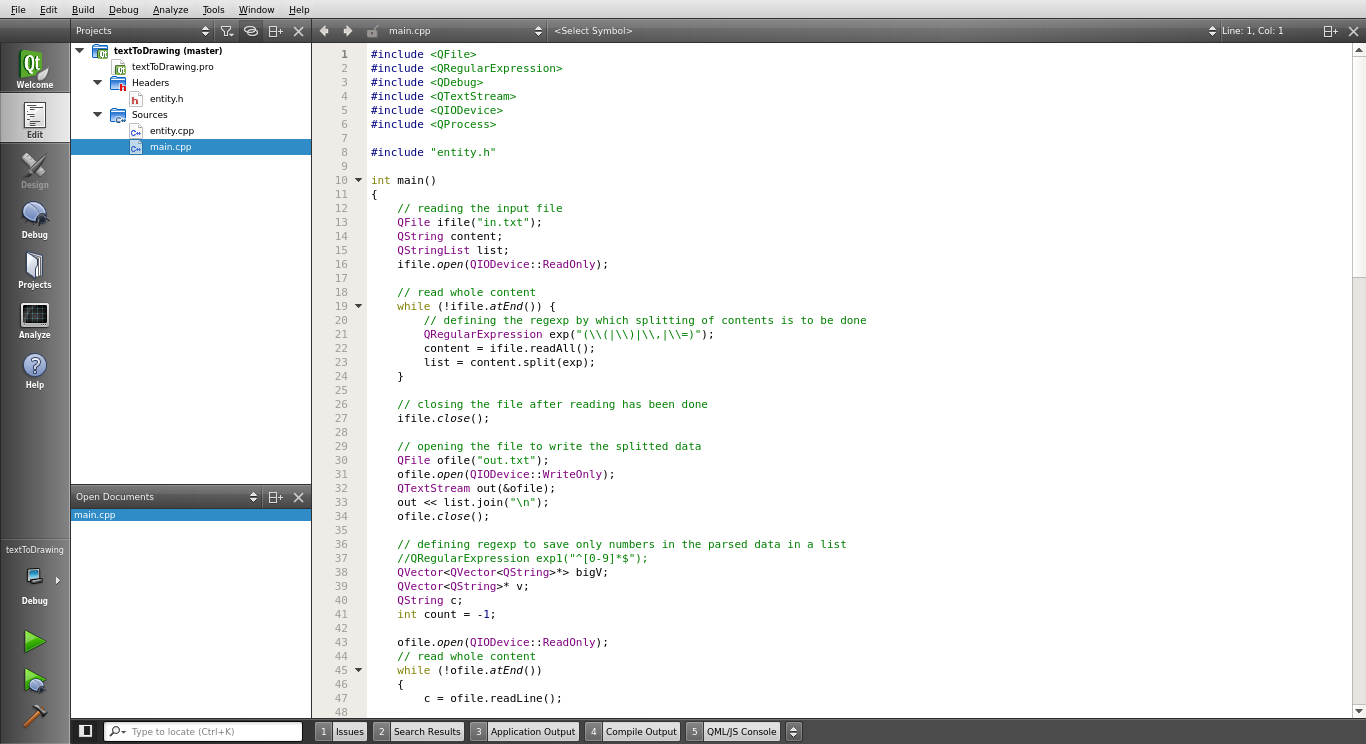
\includegraphics[scale=0.32]{images/qt-1.png}
\caption{Project opened in Qt}
\label{fig:qt}
\end{figure}

After building the project, a new file "out.txt" is generated with the separated output as shown in figure \ref{fig:cli}. It will tokenize the line from the input file and separate all tokens with a new line.

\begin{figure}
\centering
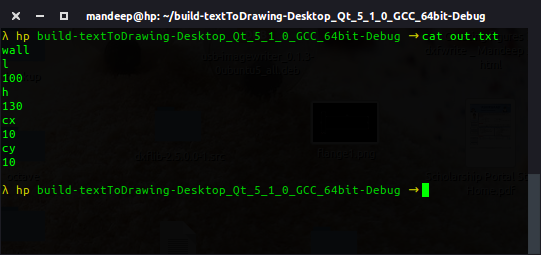
\includegraphics[scale=0.8]{images/p2.png}
\caption{Output file after tokenizing}
\label{fig:cli}
\end{figure}

If one have LibreCAD installed already on the system, then it will launch LibreCAD with the output file (DXF). Even if LibreCAD is not installed on the system, one may find the DXF file in a directory named something like Build-*. Also, one have to place the in.txt file in this directory. And it may be opened using some other CAD software of the choice of user. There are many other CAD softwares available. A popular and proprietary software AutoCAD, a free proprietary DraftSight, LibreCAD, FreeCAD, QCAD, OpenSCAD etc. Hence it depends completely on the user's choice to which software to use.

After the input being separated in "out.txt" as shown in figure \ref{fig:cli}, it's now time to view the output. The resulting dxf file is stored as myfile.dxf in the build directory in the current folder of the project. One of the output is shown in figure \ref{fig:flange}, where two walls are created using the createWall entity and a flange is created using the createFlange entity.

\begin{figure}
\centering
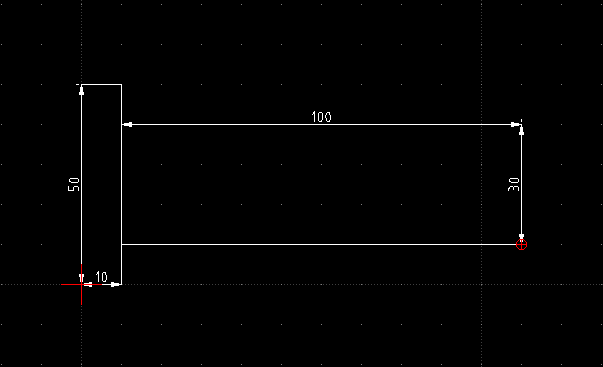
\includegraphics[scale=0.6]{images/dimensions.png}
\caption{Dimensioning example}
\label{fig:dim}
\end{figure}


\begin{figure}
\centering
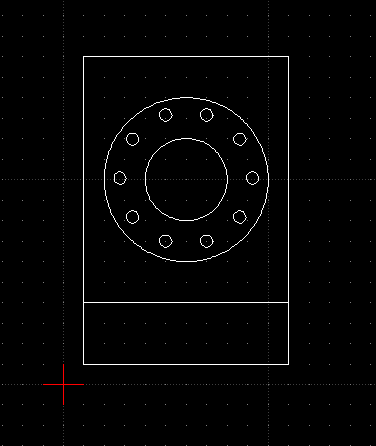
\includegraphics[scale=0.7]{images/flange.png}
\caption{A wall and flange example}
\label{fig:flange}
\end{figure}